\section{Introduction}  \label{sec:Introduction}
After observing particle interactions and correspondingly their tracks with
bubble or streamer chambers, strong increases in accuracy were required in order
to resolve reliably interaction vertices and particle paths \cite{charpak_high-resolution_1984}.
The development of detectors with electronic readout and consequently the
possibility of stacking and locating them at known positions would therefore
prove to be a working and robust solution to this problem. Strong advantages of
the gas-flow proportional counters are known already since the 1950s \cite{hendee_gasflow_1956} and include
easy read-out electronic systems and the possibility to increase detection volume
with cheaply available gas. Additionally operation at atmospheric pressure
reduces the material that charged particles need to traverse from the
interaction point as high pressure resisting walls are not required, and removes
the absolute requirement of leak-tightness as escaping gas is affordable while a
vacuum would break down.

\begin{figure}[H]
  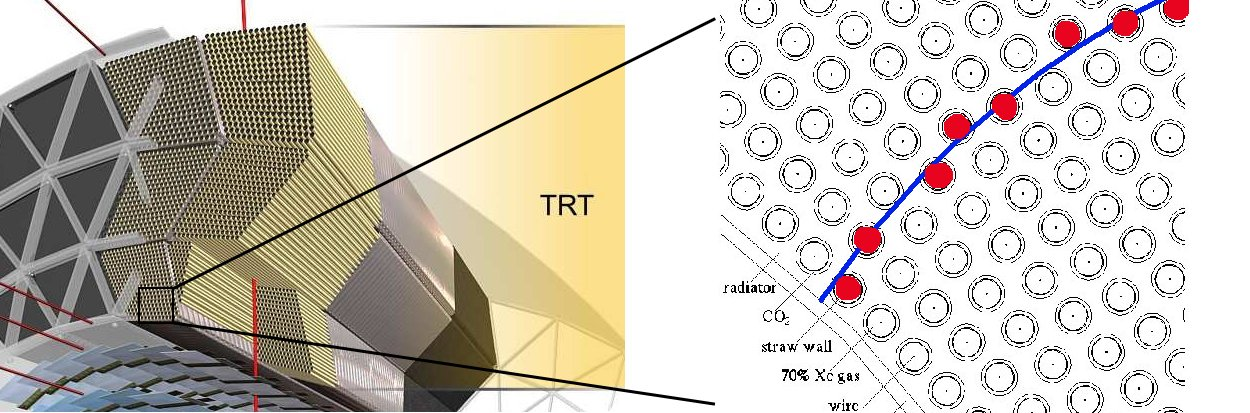
\includegraphics[width=\linewidth]{graphics/ATLAS_TRT_Principle_image}
  \caption{Principle of the ATLAS TRT using proportional counters in a specific
    arrangement. Figure taken from \cite{colliderscope}.}
  \label{fig:colliderscope}
\end{figure}

As even low amounts of signal electrons are amplified in an
avalanche that depends, among others, on the voltage applied, the gaseous
proportional counters are an effective device that can be configured towards
various application fields. It is therefore still in wide use
\cite{Mindur:2017nqn}. Figure \ref{fig:colliderscope} shows a possible
arrangement of gas proportional counters within the ATLAS transition radiation
tracker allowing to track the movement of a particle as visualized.

However with the versality of a gas detector comes along a variety of challenges
as the choice of gas, tube and wire material, voltage, amplification etc. are
all influencing the resolution and constructability of the detector. In this
laboratory we are therefore constructing a proportional counter detector from
scratch to understand the challenges that come along with the construction
process itself. Furthermore we are calibrating our detector and examine which
environmental impacts, such as the atmospheric pressure are influencing its
performance. The final objective is to measure the decay spectra of two samples:
\emph{Iron} and \emph{Americium}. In order to do this we first calibrate our self-made
detector and determine for both samples i.e. energy ranges the optimal
resolution for combinations of voltages and amplifications. We present the final
spectra and account for systematic and statistical uncertainties.